\begin{figure*}
  \centering
  \begin{subfigure}[t]{0.43\linewidth}
    \centering
  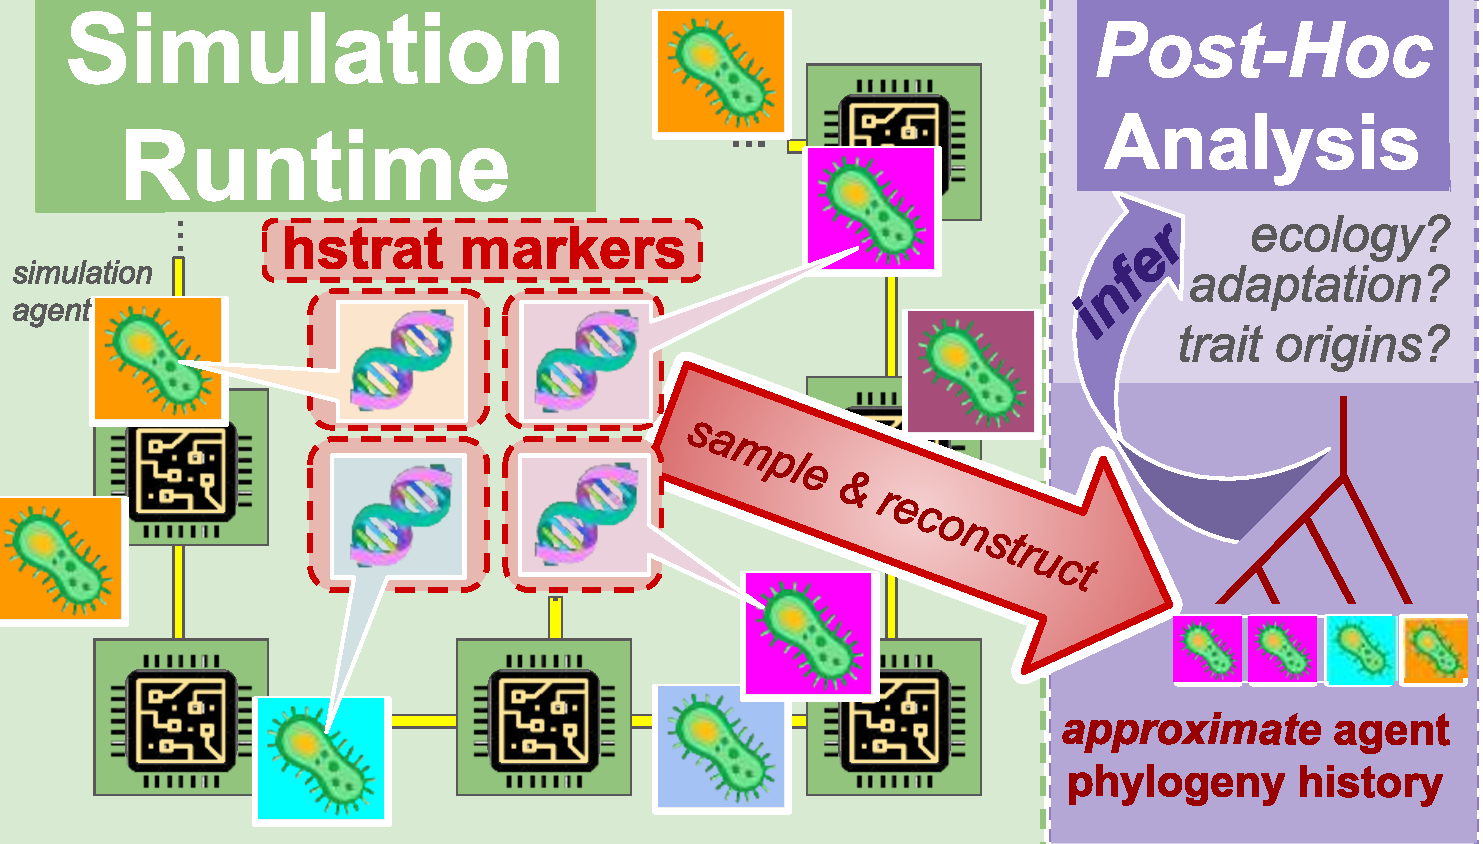
\includegraphics[width=\linewidth]{binder-wse-sketches/tex-access-proposal/img/runtime-posthoc-schematic}
    \caption{%
    Use of hstrat markers to estimate phylogenetic history and, thereby, infer evolutionary dynamics.
    }
    \label{fig:runtime-posthoc-schematic}
  \end{subfigure}
  \hspace{0.07\linewidth}
  \begin{subfigure}[t]{0.43\linewidth}
    \centering
  \includegraphics[width=\linewidth]{binder-wse-sketches/tex-access-proposal/img/async-ga-schematic}
    \caption{WSE island model evolutionary algorithm implementation.}
    \label{fig:async-ga-schematic}
  \end{subfigure}

\caption{%
\textbf{Methods for distributed evolution simulation.}
\footnotesize
Subfigure \ref{fig:runtime-posthoc-schematic} shows use of hstrat markers to for reconstruct-based phylogenetic tracking of highly-distributed evolution simulations.
Subfigure \ref{fig:async-ga-schematic} summarizes asynchronous, callback-based approach to population exchange (``migration''') used to instantiate evolving populations across WSE PEs.
}
\label{fig:schematic}

\end{figure*}
